%%%%%%%%%%%%%%%%%%%%%%%%%%%%%%%%%%%%%%%%%%%%%%%%%%%%%
%%% Task 1 %%%%%%%%%%%%%%%%%%%%%%%%%%%%%%%%%%%%%%%%%%
%%%%%%%%%%%%%%%%%%%%%%%%%%%%%%%%%%%%%%%%%%%%%%%%%%%%%
\task{Design of a singe phase transformer}

%%%%%%%%%%%%%%%%%%%%%%%%%%%%%%%%%%%%%%%%%%%%%%
\taskGerman{Auslegung eines Einphasentransformators}
%%%%%%%%%%%%%%%%%%%%%%%%%%%%%%%%%%%%%%%%%%%%%%

An (older) smartphone charger is constructed as shown in \autoref{fig:charger}. The input (grid) voltage at the transformer is $U_\mathrm{1} = \SI{230}{\volt}$. The output voltage of the charger should have an average voltage of $U_\mathrm{out} = \SI{5}{\volt}$. The rectifier causes an average voltage drop of $U_\mathrm{rectifier} = \SI{0.7}{\volt}$ between $U_2$ and $U_\mathrm{out}$. The transformer has a rated apparent power of $\SI{100}{\volt\ampere}$.

\begin{germanblock}
	Ein (älteres) Smartphone-Ladegerät ist gemäß \autoref{fig:charger} aufgebaut. Die (Netz) Eingangsspannung am Transformator beträgt $U_\mathrm{1} = \SI{230}{\volt}$. Die Ausgangsspannung des Ladegeräts soll eine mittlere Spannung von $U_\mathrm{out} = \SI{5}{\volt}$ aufweisen. Der Gleichrichter verursacht eine mittlere Spannungsdifferenz von $U_\mathrm{rectifier} = \SI{0,7}{\volt}$ zwischen $U_2$ und $U_\mathrm{out}$. Der Transformator hat eine Scheinleistung von $\SI{100}{\volt\ampere}$.
\end{germanblock}

\begin{figure}[h!]
	\centering
	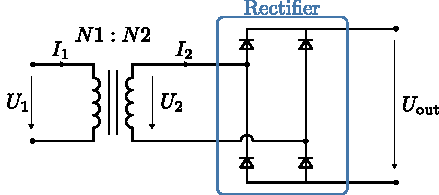
\includegraphics[scale=1.2]{fig/charger.pdf}
	\caption{Simplified sketch of a smartphone charger.}
	\label{fig:charger}
\end{figure}

\subtask{Calculate the secondary voltage, the turns ratio as well as the primary and secondary current of the transformer for rated and idealized conditions.}{2}
\begin{hintblock}
	if and only if you are not able to solve this task, use $I_\mathrm{1} = \SI{0.6}{\ampere}$, $I_\mathrm{2} = \SI{21}{\ampere}$ and $ü = 35$ as substitute results for the subsequent tasks.
\end{hintblock}

\subtaskGerman{Berechnen Sie die Sekundärspannung, das Übersetzungsverhältnis sowie den Primär- und Sek\-un\-där\-strom des Transformators für die Nennleistung unter idealisierten Bedingungen.}

\begin{germanhintblock}
	nur für den Fall, dass Sie kein Ergebnis ermitteln können, verwenden Sie $I_\mathrm{1} = \SI{0.6}{\ampere}$, $I_\mathrm{2} = \SI{21}{\ampere}$ und $ü = 35$ für die nachfolgenden Aufgaben.
\end{germanhintblock}

\begin{solutionblock}
	The secondary voltage is calculated by
	$$ U_\mathrm{2} = U_\mathrm{out} + U_\mathrm{rectifier}
		= \SI{5}{\volt} + \SI{0.7}{\volt} = \SI{5.7}{\volt},
	$$
	resulting in the transformation ratio of:
	$$ ü = \frac{N_1}{N_2} = \frac{U_1}{U_2} = 40.35.$$

	The primary current is given by
	$$ I_\mathrm{1} = \frac{S}{U_\mathrm{1}} = \SI{0.43}{\ampere},$$
	and, the secondary current is calculated by:
	$$ I_\mathrm{2} = \frac{S}{U_\mathrm{2}} = \SI{17.54}{\ampere}.$$

\end{solutionblock}

\subtask{The transformer's geometry and design is to be analyzed in more detail. The laminated core is specified as EI 84/43.5 with a magnetic flux density of $B_\mathrm{Fe} = \SI{1.2}{\tesla}$ in the middle yoke. There are no stray fluxes, and the output voltage remains constant when the transformer is loaded. Calculate the effective cross-sectional area $A_\mathrm{Fe}$ of the iron yoke, the magnetic flux $\phi_\mathrm{Fe}$ and the magnetomotive force $\theta$. The geometry and its dimensions are shown in \autoref{fig:EI_core}.}{3}
\begin{hintblock}
	if and only if you are not able to solve this task, use $\theta = \SI{100}{\ampere}$ as a substitute result for the subsequent tasks.
\end{hintblock}
\subtaskGerman{Zur Auslegung des Transformators wird nun die Geometrie genauer analysiert. Das Blechpaket ist mit EI 84/43,5 und einer Flussdichte $B_\mathrm{Fe} = \SI{1.2}{\tesla}$ im Mittelschenkel angegeben. Es gibt keine Streuflüsse, und die Ausgangsspannung bleibe bei Belastung des Transformators konstant. Berechnen Sie die effektive Querschnittsfläche $A_\mathrm{Fe}$ des Eisenjochs, den magnetischen Fluss $\phi_\mathrm{Fe}$ und die magnetische Spannung $\theta$. Die Geometrie und deren Abmessungen ist in \autoref{fig:EI_core} dargestellt.}

\begin{germanhintblock}
	nur für den Fall, dass Sie kein Ergebnis ermitteln können, verwenden Sie $\theta = \SI{100}{\ampere}$ für die nachfolgenden Aufgaben.
\end{germanhintblock}

\begin{figure}[htb]
	\begin{subfigure}{.49\textwidth}
		\centering
		% 
% \begin{figure}[htb]
% \centering
\begin{tikzpicture}[scale=.8]

	\def\a{150/20}
	\def\b{100/20}
	\def\c{25/20}
	\def\e{75/20}
	\def\delta{0/20}
	\def\threeD{10/20}

	% I-core
	\draw[thick,fill=gray!15] (0,{-\b-\delta}) -- (\a,{-\b-\delta})
	-- (\a,{-\b-\delta-\c})  -- (0,{-\b-\delta-\c}) -- (0,{-\b-\delta});

	\draw[thick,fill=gray!15,rounded corners=1pt] (0,{-\b-\delta}) -- ({cos(45)*\threeD},{sin(45)*\threeD-\b-\delta}) -- ({cos(45)*\threeD+\a},{sin(45)*\threeD-\b-\delta}) -- ({\a},{-\b-\delta}) -- ({0},{-\b-\delta});

	\draw[thick,fill=gray!15,rounded corners=1pt] (\a,{-\b-\delta-\c}) -- (\a,{-\b-\delta}) -- ({\a+cos(45)*\threeD},{-\b-\delta+sin(45)*\threeD}) -- ({\a+cos(45)*\threeD},{-\b-\delta-\c+sin(45)*\threeD}) -- (\a,{-\b-\c-\delta});

	% E-core
	\draw[thick,fill=gray!15]
	(0,0) -- (\a,0)
	-- (\a,-\b)
	-- ({\a-\c},-\b)
	-- ({\a-\c},{-\b+\e})
	-- ({\a-2*\c},{-\b+\e})
	-- ({\a-2*\c},{-\b})
	-- ({\a-4*\c},{-\b})
	-- ({\a-4*\c},{-\b+\e})
	-- ({\a-5*\c},{-\b+\e})
	-- ({\a-5*\c},{-\b})
	-- ({\a-6*\c},{-\b})
	-- ({\a-6*\c},0);

	\draw[thick,fill=gray!15,rounded corners=1pt]
	(0,0) -- ({cos(45)*\threeD},{sin(45)*\threeD}) -- ({cos(45)*\threeD+\a},{sin(45)*\threeD}) -- (\a,0) -- (0,0);

	\draw[thick,fill=gray!15,rounded corners=1pt] (\a,-\b) -- (\a,0) --({cos(45)*\threeD+\a},{sin(45)*\threeD}) -- ({cos(45)*\threeD+\a},{sin(45)*\threeD-\b}) -- (\a,-\b);

	\draw[thick,fill=gray!15,rounded corners=1pt] ({\a-5*\c},{-\b}) -- ({\a-5*\c},{-\b+\e}) -- ({\a-5*\c+cos(45)*\threeD},{-\b+\e}) -- ({\a-5*\c+cos(45)*\threeD},{-\b+sin(45)*\threeD}) -- ({\a-5*\c},{-\b});

	\draw[thick,fill=gray!15,rounded corners=1pt] ({\a-2*\c},{-\b}) -- ({\a-2*\c},{-\b+\e}) -- ({\a-2*\c+cos(45)*\threeD},{-\b+\e}) -- ({\a-2*\c+cos(45)*\threeD},{-\b+sin(45)*\threeD}) -- ({\a-2*\c},{-\b});

	% a
	\draw[|<->|] ({cos(45)*\threeD},{sin(45)*\threeD+0.2}) -- ({cos(45)*\threeD+\a},{sin(45)*\threeD+0.2}) node[midway, above] {$a = 84\,\text{mm}$};
	% b
	\draw[|<->|] (-.2,0) -- (-.2,-\b) node[midway, above, rotate=90] {$b = 56\,\text{mm}$};
	% f
	\draw[|<->] ({\a-2*\c},-1) -- ({\a-4*\c},-1) node[midway, above] {$d = 28\,\text{mm}$};
	% g
	\draw[|<->|] ({\a-4*\c},-1) -- ({\a-5*\c},-1) node[left, above] {$g = 14\,\text{mm}$};
	% c
	\draw[|<->|] ({\a},-1) -- ({\a-\c},-1) node[midway, above] {$c$};
	% c in I-core
	\draw[|<->|] ({\a/9},{-\b-\delta}) -- ({\a/9},{-\b-\delta-\c}) node[midway, right] {$c= 14\,\text{mm}$};

	% e
	\draw[<->] ({\a/4*3.2},{-\b+\e}) -- ({\a/4*3.2},{-\b}) node[midway, above, rotate=90] {$e= 42\,\text{mm}$};
	\draw[-|] ({\a/4*3.2},{-\b}) -- ({\a/4*3.2},{-\b});

	% w
	\draw[>|-|<] ({\a},{-\b-\c-.4})--({\a + \threeD*cos(45)+.4},{-\b -\c -.4 +\threeD*sin(45)+.4}) node[left, below, rotate=45]{$w= 43.5\,\text{mm}$} ;

	% average field length
	\draw[dashed] ({\a-\c/2},-\c) -- ({\a-\c/2},-\b-\c/2-\delta) -- ({\a-2*\c-\c/2},-\b-\c/2-\delta) --({\a-2*\c-\c/2},-\c);
	\draw[dashed] ({\a-\c},-\c/2) --({\a-2*\c},-\c/2);
	\draw[thin] ({\a-\c/2},-\b/2) -- ({\a+\c/2},-\b/3) node[right] {$l_\mathrm{m}$};

	\tikzmath{
		real \lx, \ly, \dr;
		\lx = 2*\c;
		\ly = -\b;
		\dr = 0.02;
	}

	\def\zz{0.24}
	\draw [rounded corners=2pt,signalblue, thick]
	({2*\c-0.09},{\ly+\zz}) -- (\lx, {\ly+\zz})--++({2*\c+0.43},0.5)
	--++(-0.08, 0.05);

	\foreach \z in {.48,.72,...,2.25}
		{
			\draw [rounded corners=2pt,signalblue, thick]
			({2*\c},\ly+\z+0.08)--({2*\c-0.09},\ly+\z) -- (\lx, \ly+\z)--++({2*\c+0.43},0.5)
			--++(-0.08, 0.05);
		}

	\def\zz{2.4}
	\draw [rounded corners=2pt,signalblue, thick]
	({2*\c-0.09},{\ly+\zz}) -- (\lx, {\ly+\zz})--++({2*\c+0.43},0.5)
	--++(-0.08, 0.05);

	\draw[thick,signalblue](2.5,{-\b+0.24}) -- (2,{-\b+0.24});
	\draw[thick,signalblue](2.5,{-\b+2.4}) -- (2,{-\b+2.4});

	\draw [thick,signalblue, <-](2.5,{-\b+0.24}) -- (2,{-\b+0.24});

\end{tikzpicture}
% \caption{Sketch of the EI-150 core.}
% \label{fig:EI_core}
% \end{figure}
		\caption{EI-84/43.5 core geometry.}
		\label{fig:EI_core_sketch}
	\end{subfigure}
	\begin{subfigure}{.49\textwidth}
		\centering
		\input{./fig/magnetization.tex}
		\caption{Magnetization curve.}
		\label{fig:magnetization_curve}
	\end{subfigure}
	\caption{EI-84/43.5 core and electrical steel magnetization curve.}
	\label{fig:EI_core}
\end{figure}

\begin{solutionblock}
	The cross sectional area is given with:
	$$ A_\mathrm{Fe} = d  w = \SI{0.0012}{\metre^2}. $$
	Thus, the magnetic flux is calculated as
	$$ \phi_\mathrm{Fe} = B_\mathrm{fe} A_\mathrm{Fe} = \SI{0.00146}{\weber}, $$
	and, the magnetic field can be taken from the magnetization curve, which is $H_\mathrm{Fe} = \SI{500}{\ampere\per\metre}$.

	The average length of the magnetic path in the E-core is given by
	$$ l_\mathrm{E} =  2 e + g + 2c = \SI{0.126}{\metre},$$
	and for the I-core as
	$$ l_\mathrm{I} = 2c +g = \SI{0.042}{\metre}.$$
	Thus, the average length of the magnetic path is given with
	$$ l_\mathrm{m} = l_\mathrm{E} + l_\mathrm{I} = \SI{0.168}{\metre}, $$
	therefore, the magnetomotive force is calculated as
	$$ \theta = H_\mathrm{Fe} l_\mathrm{m} = \SI{84}{\ampere}.$$

\end{solutionblock}

\subtask{Calculate the integer number of winding turns on the primary and secondary side.} {1}

\subtaskGerman{Berechnen Sie die ganzzahlige Anzahl der Windungen auf der Primär- und Sekundärseite.}

\begin{solutionblock}
	The primary winding turns are calculated by
	$$ N_\mathrm{1} = \frac{\theta}{I_\mathrm{1}}  = 193.2, $$
	and, for the secondary side as
	$$ N_\mathrm{2} = \frac{N_\mathrm{1}}{ü} = 4.78,$$
	which results in $N_\mathrm{1} = 193$ and $N_\mathrm{2} = 5$ turns, respectively.
\end{solutionblock}

\subtask{Determine the ohmic winding losses and wire diameters of the primary and secondary sides. First calculate the winding cross-sections assuming a current density of $J = \SI{3}{\ampere\per\milli\metre^2}$, an average turn length of $l_\mathrm{w} = \SI{0.25}{\metre}$, and an electrical conductivity of $\kappa_\mathrm{Cu} = \SI{50\cdot 10^6}{\siemens\per\metre}$.}{3}

\subtaskGerman{Bestimmen Sie die ohmschen Verluste der Wicklungen und den Drahtdurchmesser auf der Primär- und Sekundärseite. Beginnen Sie mit der Berechnung des Querschnitts der Wicklungen unter der Annahme einer Stromdichte von $J = \SI{3}{\ampere\per\milli\metre^2}$ und einer durchschnittlichen Wickellänge pro Windung von $l_\mathrm{w} = \SI{0.25}{\metre}$. Die elektrische Leitfähigkeit ist mit $\kappa_\mathrm{Cu} = \SI{50\cdot 10^6}{\siemens\per\metre}$ gegeben.}

\begin{solutionblock}
	The cross section is given by:
	$$ q_\mathrm{1} = \frac{I_\mathrm{1}}{J} = \SI{0.145\cdot10^{-6}}{\metre^2},$$
	and, $q_\mathrm{2} = \SI{5.85\cdot10{^-6}}{\metre^2}$, respectively. The resistance is calculated with
	$$ R_\mathrm{1} = \frac{1}{\kappa_\mathrm{Cu}} \frac{N_\mathrm{1}}{q_\mathrm{1}} l_\mathrm{w} = \SI{6.66}{\Omega},$$
	and $R_\mathrm{2} = \SI{0.004}{\Omega}$, respectively. The wire diameters are calculated by
	$$ d_\mathrm{1} = 2 \sqrt{\frac{q_\mathrm{1}}{\pi}} = \SI{0.42}{\milli\metre},$$
	and $d_\mathrm{2} = \SI{2.73}{\milli\metre}$. With the winding resistance, the cupper losses result in
	$$ P_\mathrm{1} = I_\mathrm{1}^2 R_\mathrm{1} = \SI{1.26}{\watt},$$
	and,
	$P_\mathrm{2} = \SI{1.32}{\watt}$.

\end{solutionblock}

\subtask{To also charge a laptop with a battery voltage of \SI{12}{\volt}, which transformer type would allow one charger to provide both output voltages?}{1}
\begin{hintblock}
	This task is independent of the previous tasks and can be solved qualitatively without reference to the previous results.
\end{hintblock}
\subtaskGerman{Sie möchten nun auch einen Laptop mit einer Batteriespannung von \SI{12}{\volt} laden. Welche Transformatorart ist geeignet, damit das Ladegerät beide Ausgangsspannungen bereitstellen kann?}

\begin{germanhintblock}
	Diese Aufgabe ist unabhängig von den vorherigen Aufgaben und kann qualitativ ohne Bezug auf die vorherigen Ergebnisse gelöst werden.
\end{germanhintblock}

\begin{solutionblock}
	In this case a tap transformer could be used, which has two taps on the secondary winding, allowing to select between the different output voltages. The required output voltage can be selected by a switch that connects the two windings to the rectifier.
\end{solutionblock}